%set the master document for easy compilation
%!TEX root = ../D3_5_3.tex

\section{F2.2: Manage\_ETCS\_Procedures}\label{s:F2.2}



\subsection{Component Requirements}

\begin{longtable}{p{.25\textwidth}p{.7\textwidth}}
\toprule
Component name			& Manage\_ETCS\_Procedures \\
\midrule
Link to SCADE model		& {\footnotesize \url{https://github.com/openETCS/modeling/tree/master/model/Scade/System/ObuFunctions/Procedures}} \\
\midrule
SCADE designer			&  Baseliyos Jacob, DB Netz AG\\
\midrule
Description				& This function describes the Start of Mission procedure of the train until the current status will change to another mode, level or other procedure. \\
\midrule
Input documents	& 
Subset-026, Chapter 5.4\\
\midrule
Safety integrity level		& 4 \\
\midrule
Time constraints		& n/a \\
\midrule
API requirements 		& n/a \\
\bottomrule
\end{longtable}


\subsection{Interface}

An overview of the interface of component Manage\_ETCS\_Procedures is shown in Figure~\ref{f:etcs_procedures_interface}. The inputs and outputs are described in detail in Section~\ref{s:etcs_procedures_inputs} respectively \ref{s:etcs_procedures_outputs}. Subcomponents are described in Section~\ref{s:etcs_procedures_subcomponents}.

\begin{figure}
\center
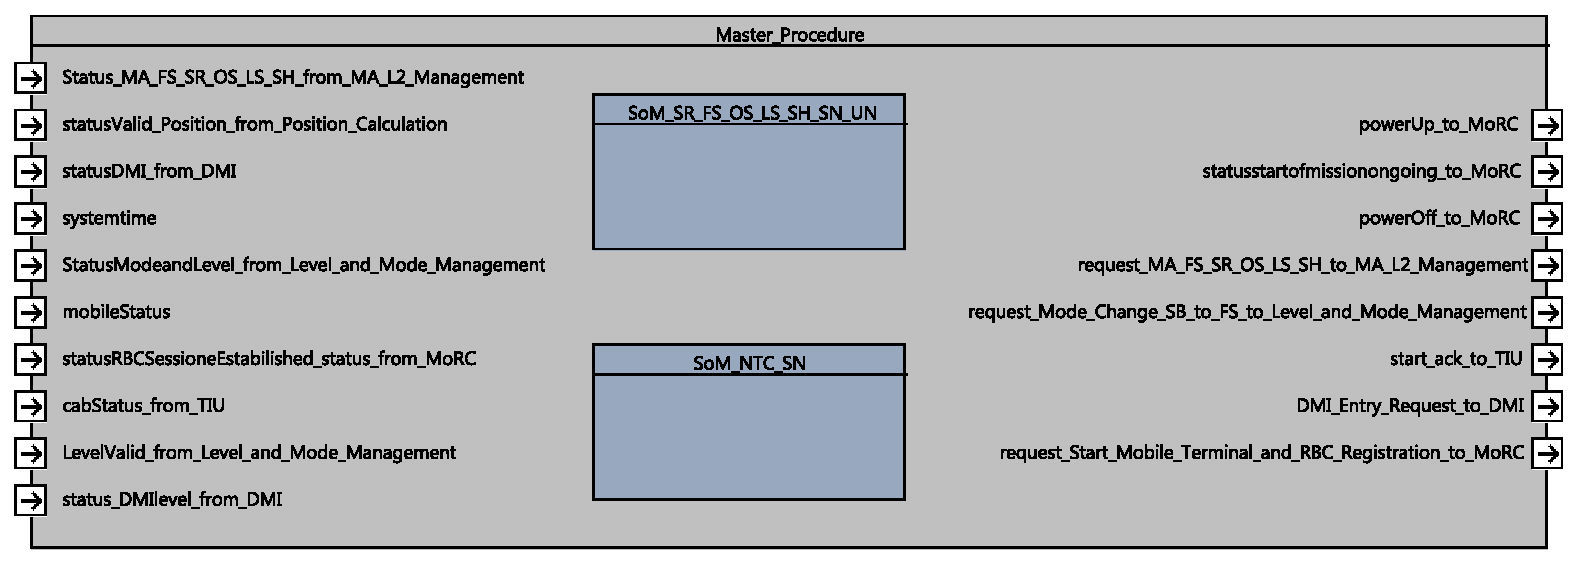
\includegraphics[width=\textwidth]{images/F2_2_Manage_ETCS_Procedures.pdf}
\caption{Manage\_ETCS\_Procedures component SysML diagram.}\label{f:etcs_procedures_interface}
\end{figure}


\subsubsection{Inputs}\label{s:etcs_procedures_inputs}

\paragraph{statusDMI\_from\_DMI}

\begin{longtable}{p{.25\textwidth}p{.7\textwidth}}
\toprule
Input name				& statusDMI\_from\_DMI \\
\midrule
Description				& Input interface of DMI Controller status. \\
\midrule
Source					& F2.10 manageDMI\_input  \\ 
\midrule
Type					& DMI\_Types\_Pkg::DMI\_EVC\_status\_T \\
\midrule
Valid range of values	& See SCADE generated documentation respectively SCADE Suite functional model. \\
\midrule
Behaviour when value is at boundary	& n/a \\
\midrule
Behaviour for values out of valid range	& Function will not be triggered. \\
\midrule
Behaviour when value is erroneous, absent or unwanted (i.e. spurious) & Function will not be triggered. \\
\bottomrule
\end{longtable}


\paragraph{Status\_MA\_FS\_SR\_OS\_LS\_SH\_from\_MA\_L2\_Management}

\begin{longtable}{p{.25\textwidth}p{.7\textwidth}}
\toprule
Input name				& Status\_MA\_FS\_SR\_OS\_LS\_SH\_from\_MA\_L2\_Management \\
\midrule
Description				& Status of MA, Mode and Level from Level and Mode Management. \\
\midrule
Source					& F2.2 Manage\_ETCS\_Procedures \\ 
\midrule
Type					& bool \\
\midrule
Valid range of values	& \begin{description}
\item[true]Movement Authority for Level 2 FS is valid
\item[false]Movement Authority for Level 2 FS is not valid
\end{description} \\
\midrule
Behaviour when value is at boundary	& n/a \\
\midrule
Behaviour for values out of valid range	& n/a \\
\midrule
Behaviour when value is erroneous, absent or unwanted (i.e. spurious) & n/a \\
\bottomrule
\end{longtable}

\paragraph{systemtime}

\begin{longtable}{p{.25\textwidth}p{.7\textwidth}}
\toprule
Input name				& systemtime \\
\midrule
Description				& Standardized system time used for all internal calculations. \\
\midrule
Source					& F2 input API\_Systemtime \\ 
\midrule
Type					& Obu\_BasicTypes\_Pkg::T\_internal\_Type \\
\midrule
Valid range of values	& 
$[0,\text{maximum positive int value of target platform}]$ \\
\midrule
Behaviour when value is at boundary	& System time is assumed to be valid. \\
\midrule
Behaviour for values out of valid range	& System time is assumed to be valid. \\
\midrule
Behaviour when value is erroneous, absent or unwanted (i.e. spurious) & System time is assumed to be valid. \\
\bottomrule
\end{longtable}

\paragraph{StatusModeandLevel\_from\_Level\_and\_Mode\_Management}

\begin{longtable}{p{.25\textwidth}p{.7\textwidth}}
\toprule
Input name				& StatusModeandLevel\_from\_Level\_and\_Mode\_Management  \\
\midrule
Description				& Status of Mode and Level. \\
\midrule
Source					& F2.10 ManageLevelAndMode \\ 
\midrule
Type					& Level\_And\_Mode\_Types\_Pkg::T\_Mode\_Level \\
\midrule
Valid range of values	& See SCADE generated documentation respectively SCADE Suite functional model. \\
\midrule
Behaviour when value is at boundary	& n/a \\
\midrule
Behaviour for values out of valid range	& n/a \\
\midrule
Behaviour when value is erroneous, absent or unwanted (i.e. spurious) & n/a \\
\bottomrule
\end{longtable}

\paragraph{mobileSwStatus\_p\_from\_MoRC}

\begin{longtable}{p{.25\textwidth}p{.7\textwidth}}
\toprule
Input name				& mobileSwStatus\_p\_from\_MoRC  \\
\midrule
Description				& Information about SW status from Management of Radio Communication function. \\
\midrule
Source					& F2.9 MoRC\_HO\\ 
\midrule
Type					& MoRC\_Pck::mobileSWStatus\_Type \\
\midrule
Valid range of values	& See SCADE generated documentation respectively SCADE Suite functional model. \\
\midrule
Behaviour when value is at boundary	&n/a \\
\midrule
Behaviour for values out of valid range	& n/a \\
\midrule
Behaviour when value is erroneous, absent or unwanted (i.e. spurious) & n/a \\
\bottomrule
\end{longtable}

\paragraph{statusRBCSessioneEstabilished\_status\_from\_MoRC}

\begin{longtable}{p{.25\textwidth}p{.7\textwidth}}
\toprule
Input name				& statusRBCSessioneEstabilished\_status\_from\_MoRC  \\
\midrule
Description				& Information about RBC Session status from the Management of Radio Communication function. \\
\midrule
Source					&  F2.9 MoRC\_HO\\ 
\midrule
Type					& Radio\_Types\_Pkg::sessionStatus\_Type \\
\midrule
Valid range of values	& See SCADE generated documentation respectively SCADE Suite functional model. \\
\midrule
Behaviour when value is at boundary	& n/a \\
\midrule
Behaviour for values out of valid range	& n/a \\
\midrule
Behaviour when value is erroneous, absent or unwanted (i.e. spurious) & n/a \\
\bottomrule
\end{longtable}

\paragraph{cabStatus\_from\_TIU}

\begin{longtable}{p{.25\textwidth}p{.7\textwidth}}
\toprule
Input name				& cabStatus\_from\_TIU  \\
\midrule
Description				& Information about cab desk status from Train Interface Unit function. \\
\midrule
Source					& F2.12 manageTIU\_input\\ 
\midrule
Type					& TIU\_Types\_Pkg::TIU\_trainStatus\_T \\
\midrule
Valid range of values	& See SCADE generated documentation respectively SCADE Suite functional model. \\
\midrule
Behaviour when value is at boundary	& n/a \\
\midrule
Behaviour for values out of valid range	& n/a \\
\midrule
Behaviour when value is erroneous, absent or unwanted (i.e. spurious) & n/a \\
\bottomrule
\end{longtable}

\paragraph{statusValid\_Position\_from\_Position\_Calculation}

\begin{longtable}{p{.25\textwidth}p{.7\textwidth}}
\toprule
Input name				& statusValid\_Position\_from\_Position\_Calculation  \\
\midrule
Description				& Information about validity status of the train position calculation. \\
\midrule
Source					& F2.6 calculateTrainPosition\\ 
\midrule
Type					& bool \\
\midrule
Valid range of values	& \begin{description}
\item[true]Calculated train position is valid.
\item[false]Calculated train position is not valid.
\end{description} \\
\midrule
Behaviour when value is at boundary	& n/a \\
\midrule
Behaviour for values out of valid range	& n/a\\
\midrule
Behaviour when value is erroneous, absent or unwanted (i.e. spurious) & n/a \\
\bottomrule
\end{longtable}

\paragraph{status\_DMIlevel\_from\_DMI}

\begin{longtable}{p{.25\textwidth}p{.7\textwidth}}
\toprule
Input name				& status\_DMIlevel\_from\_DMI  \\
\midrule
Description				& Information about the status of DMI menu and level request from DMIController function. \\
\midrule
Source					& F2.10 manageDMI\_input\\ 
\midrule
Type					& DMI\_Messages\_DMI\_to\_EVC\_Pkg::DMI\_Driver\_Request\_T \\
\midrule
Valid range of values	& See SCADE generated documentation respectively SCADE Suite functional model. \\
\midrule
Behaviour when value is at boundary	& n/a \\
\midrule
Behaviour for values out of valid range	& n/a \\
\midrule
Behaviour when value is erroneous, absent or unwanted (i.e. spurious) & n/a \\
\bottomrule
\end{longtable}

\paragraph{LevelValid\_from\_Level\_and\_Mode\_Management}

\begin{longtable}{p{.25\textwidth}p{.7\textwidth}}
\toprule
Input name				& LevelValid\_from\_Level\_and\_Mode\_Management  \\
\midrule
Description				& Information about the validty status of  the StatusModeandLevel\_from\_Level\_and\_Mode\_Management input. \\
\midrule
Source					& F2.5 ManageModeAndLevel \\
\midrule
Type					& bool \\
\midrule
Valid range of values	& \begin{description}
\item[true]Level and Mode information are valid.
\item[false]Level and Mode information are not valid.
\end{description} \\
\midrule
Behaviour when value is at boundary	& n/a \\
\midrule
Behaviour for values out of valid range	& n/a\\
\midrule
Behaviour when value is erroneous, absent or unwanted (i.e. spurious) & n/a \\
\bottomrule
\end{longtable}

\subsubsection{Outputs}\label{s:etcs_procedures_outputs}

\paragraph{DMI\_Entry\_Request\_to\_DMI}

\begin{longtable}{p{.25\textwidth}p{.7\textwidth}}
\toprule
Output name				& DMI\_Entry\_Request\_to\_DMI \\
\midrule
Description				& Information about input request to the driver. \\
\midrule
Destination				& F2.11 manageDMI\_output \\ 
\midrule
Type					& DMI\_Messages\_EVC\_to\_DMI\_Pkg::DMI\_Entry\_Request\_T \\
\midrule
Valid range of values	& See SCADE generated documentation respectively SCADE Suite functional model. \\
\midrule
Behaviour when value is at boundary	& n/a \\
\midrule
Behaviour for values out of valid range	& n/a \\
\midrule
Behaviour when value is erroneous, absent or unwanted (i.e. spurious) & n/a \\
\bottomrule
\end{longtable}

\paragraph{request\_Start\_Mobile\_Terminal\_and\_RBC\_Registration\_to\_MoRC}

\begin{longtable}{p{.25\textwidth}p{.7\textwidth}}
\toprule
Output name				& request\_Start\_Mobile\_Terminal\_and\_RBC\_Registration\_to\_MoRC \\
\midrule
Description				& This output is a trigger to start the mobile terminal and RBC session registration within the Management of Radio Communication function. \\
\midrule
Destination				& F2.9 MoRC\_HI \\
\midrule
Type					& Common\_Types\_Pkg::radioManagementMessage\_T \\
\midrule
Valid range of values	& See SCADE generated documentation respectively SCADE Suite functional model. \\
\midrule
Behaviour when value is at boundary	& n/a \\
\midrule
Behaviour for values out of valid range	& n/A \\
\midrule
Behaviour when value is erroneous, absent or unwanted (i.e. spurious) & n/a \\
\bottomrule
\end{longtable}

\paragraph{powerUp\_to\_MoRC}

\begin{longtable}{p{.25\textwidth}p{.7\textwidth}}
\toprule
Output name				& powerUp\_to\_MoRC \\
\midrule
Description				& This output is the trigger to activate the Management of Radio Communication function. \\
\midrule
Destination				& F2.9 MoRC\_HO \\ 
\midrule
Type					& bool \\
\midrule
Valid range of values	& \begin{description}
\item[true]MoRC will be activated. 
\item[false]No action.
\end{description} \\
\midrule
Behaviour when value is at boundary	& n/a \\
\midrule
Behaviour for values out of valid range	& n/a \\
\midrule
Behaviour when value is erroneous, absent or unwanted (i.e. spurious) & n/a \\
\bottomrule
\end{longtable}

\paragraph{statusstartofmissionongoing\_to\_MoRC}

\begin{longtable}{p{.25\textwidth}p{.7\textwidth}}
\toprule
Output name				& statusstartofmissionongoing\_to\_MoRC \\
\midrule
Description				& This output gives the information about the start of mission status procedure to the Management of Radio Communication function. \\
\midrule
Destination				& F2.9 MoRC\_HO \\ 
\midrule
Type					& bool \\
\midrule
Valid range of values	& \begin{description}
\item[true]Start of mission procedure is currently ongoing.
\item[false]Start of mission procedure is currently not ongoing.
\end{description} \\
\midrule
Behaviour when value is at boundary	& n/a \\
\midrule
Behaviour for values out of valid range	& n/a \\
\midrule
Behaviour when value is erroneous, absent or unwanted (i.e. spurious) & n/a \\
\bottomrule
\end{longtable}

\paragraph{powerOff\_to\_MoRC}

\begin{longtable}{p{.25\textwidth}p{.7\textwidth}}
\toprule
Output name				& powerOff\_to\_MoRC \\
\midrule
Description				& This output is the trigger to de-activate the Management of Radio Communication function. \\
\midrule
Destination				& F2.9 MoRC\_HO \\ 
\midrule
Type					& bool \\
\midrule
Valid range of values	& \begin{description}
\item[true]MoRC will be deactivated. 
\item[false]no action.
\end{description} \\
\midrule
Behaviour when value is at boundary	& n/a \\
\midrule
Behaviour for values out of valid range	& n/a \\
\midrule
Behaviour when value is erroneous, absent or unwanted (i.e. spurious) & n/a \\
\bottomrule
\end{longtable}

\paragraph{start\_ack\_to\_TIU}

\begin{longtable}{p{.25\textwidth}p{.7\textwidth}}
\toprule
Output name				& start\_ack\_to\_TIU \\
\midrule
Description				& This output indicates that the start of mission procedure is completed. \\
\midrule
Destination				& Output is currently not used in the model. \\ 
\midrule
Type					& bool \\
\midrule
Valid range of values	&  \begin{description}
\item[true]Start of mission procedure is completed.
\item[false]Not defined. 
\end{description} \\
\midrule
Behaviour when value is at boundary	& n/a \\
\midrule
Behaviour for values out of valid range	& n/a \\
\midrule
Behaviour when value is erroneous, absent or unwanted (i.e. spurious) & n/a \\
\bottomrule
\end{longtable}


\subsection{Subcomponents}\label{s:etcs_procedures_subcomponents}

\subsubsection{Awakness\_of\_Train}
%set the master document for easy compilation
%!TEX root = ../D3_5_3.tex

\paragraph{Component Requirements}

\begin{longtable}{p{.25\textwidth}p{.7\textwidth}}
\toprule
Component name			& Awakness\_of\_Train \\
\midrule
Link to SCADE model		& {\footnotesize \url{https://github.com/openETCS/modeling/blob/master/model/Scade/System/ObuFunctions/Procedures/ManageProcedure_Pkg.xscade}} \\
\midrule
SCADE designer			& Baseliyos Jacob, DB Netz AG \\
\midrule
Description				& This component describes the Start of Mission procedure of the train until the status of the awakening is completed. From this point on the train will be able to switch to further modes, levels and procedures. \\

\midrule
Input documents	& 
Subset-026, Chapter 5, § 5.4 \\
\midrule
Safety integrity level		& 4 \\
\midrule
Time constraints		& n/a \\
\midrule
API requirements 		& n/a \\
\bottomrule
\end{longtable}



\paragraph{Interface}

For an overview of the interface of this internal component we refer to the SCADE model (cf.~link above) respectively the SCADE generated documentation.

\subsubsection{NP}
%set the master document for easy compilation
%!TEX root = ../D3_5_3.tex

\paragraph{Component Requirements}

\begin{longtable}{p{.25\textwidth}p{.7\textwidth}}
\toprule
Component name			& NP \\
\midrule
Link to SCADE model		& {\footnotesize \url{https://github.com/openETCS/modeling/blob/master/model/Scade/System/ObuFunctions/Procedures/ManageProcedure_Pkg.xscade}} \\
\midrule
SCADE designer			& Baseliyos Jacob, DB Netz AG \\
\midrule
Description				& This component implements the No Power status of the train before the driver opens the cab desk. \\

\midrule
Input documents	& 
Subset-026, Chapter 5, § 5.4 \\
\midrule
Safety integrity level		& 4 \\
\midrule
Time constraints		& n/a \\
\midrule
API requirements 		& n/a \\
\bottomrule
\end{longtable}



\paragraph{Interface}

For an overview of the interface of this internal component we refer to the SCADE model (c.f.~link above) respectively the SCADE generated documentation.

\subsubsection{SoM\_L2\_3\_FS\_SR\_OS\_LS\_SH}
%set the master document for easy compilation
%!TEX root = ../D3_5_3.tex

\paragraph{Component Requirements}

\begin{longtable}{p{.25\textwidth}p{.7\textwidth}}
\toprule
Component name			& SoM\_L2\_3\_FS\_SR\_OS\_LS\_SH \\
\midrule
Link to SCADE model		& {\footnotesize \url{https://github.com/openETCS/modeling/blob/master/model/Scade/System/ObuFunctions/Procedures/ManageProcedure_Pkg.xscade}} \\
\midrule
SCADE designer			& Baseliyos Jacob, DB Netz AG \\
\midrule
Description				& This component switch to Level 2 or 3 and Mode FS, SR, OS, LS and SH after completion of the awakening of the train. \\

\midrule
Input documents	& 
Subset-026, Chapter 5, § 5.4 \\
\midrule
Safety integrity level		& 4 \\
\midrule
Time constraints		& n/a \\
\midrule
API requirements 		& n/a \\
\bottomrule
\end{longtable}



\paragraph{Interface}

For an overview of the interface of this internal component we refer to the SCADE model (c.f.~link above) respectively the SCADE generated documentation.

\subsubsection{SoM\_NTC\_SN}
%set the master document for easy compilation
%!TEX root = ../D3_5_3.tex

\paragraph{Component Requirements}

\begin{longtable}{p{.25\textwidth}p{.7\textwidth}}
\toprule
Component name			& SoM\_NTC\_SN \\
\midrule
Link to SCADE model		& {\footnotesize \url{https://github.com/openETCS/modeling/blob/master/model/Scade/System/ObuFunctions/Procedures/ManageProcedure_Pkg.xscade}} \\
\midrule
SCADE designer			& Baseliyos Jacob, DB Netz AG \\
\midrule
Description				& This component switch to Level NTC and Mode SN after completion of the awakening of the train. \\

\midrule
Input documents	& 
Subset-026, Chapter 5, § 5.4 \\
\midrule
Safety integrity level		& 4 \\
\midrule
Time constraints		& n/a \\
\midrule
API requirements 		& n/a \\
\bottomrule
\end{longtable}



\paragraph{Interface}

For an overview of the interface of this internal component we refer to the SCADE model (c.f.~link above) respectively the SCADE generated documentation.


